%%%%%%%%%%%%%%%%%%%%%%%%%%%%%%%%%%%%%%%%%
% Journal Article
% LaTeX Template
% Version 1.4 (15/5/16)
%
% This template has been downloaded from:
% http://www.LaTeXTemplates.com
%
% Original author:
% Frits Wenneker (http://www.howtotex.com) with extensive modifications by
% Vel (vel@LaTeXTemplates.com)
%
% License:
% CC BY-NC-SA 3.0 (http://creativecommons.org/licenses/by-nc-sa/3.0/)
%
%%%%%%%%%%%%%%%%%%%%%%%%%%%%%%%%%%%%%%%%%
%----------------------------------------------------------------------------------------
%	PACKAGES AND OTHER DOCUMENT CONFIGURATIONS
%----------------------------------------------------------------------------------------

\documentclass[twoside,twocolumn]{article}

\usepackage{blindtext} % Package to generate dummy text throughout this template

\usepackage[sc]{mathpazo} % Use the Palatino font
\usepackage[utf8]{inputenc}
\usepackage[T1]{fontenc} % Use 8-bit encoding that has 256 glyphs
\linespread{1.05} % Line spacing - Palatino needs more space between lines
\usepackage{microtype} % Slightly tweak font spacing for aesthetics

\usepackage[english]{babel} % Language hyphenation and typographical rules

\usepackage[hmarginratio=1:1,top=32mm,columnsep=20pt]{geometry} % Document margins
\usepackage[hang, small,labelfont=bf,up,textfont=it,up]{caption} % Custom captions under/above floats in tables or figures
\usepackage{booktabs} % Horizontal rules in tables

\usepackage{lettrine} % The lettrine is the first enlarged letter at the beginning of the text

\usepackage{enumitem} % Customized lists
\setlist[itemize]{noitemsep} % Make itemize lists more compact

\usepackage{abstract} % Allows abstract customization
\renewcommand{\abstractnamefont}{\normalfont\bfseries} % Set the "Abstract" text to bold
\renewcommand{\abstracttextfont}{\normalfont\small\itshape} % Set the abstract itself to small italic text

\usepackage{titlesec} % Allows customization of titles
\renewcommand\thesection{\Roman{section}} % Roman numerals for the sections
\renewcommand\thesubsection{\roman{subsection}} % roman numerals for subsections
\titleformat{\section}[block]{\large\scshape\centering}{\thesection.}{1em}{} % Change the look of the section titles
\titleformat{\subsection}[block]{\large}{\thesubsection.}{1em}{} % Change the look of the section titles

\usepackage{fancyhdr} % Headers and footers
\pagestyle{fancy} % All pages have headers and footers
\fancyhead{} % Blank out the default header
\fancyfoot{} % Blank out the default footer
\fancyhead[C]{Running title $\bullet$ May 2016} % Custom header text
\fancyfoot[RO,LE]{\thepage} % Custom footer text

\usepackage{titling} % Customizing the title section

\usepackage{hyperref} % For hyperlinks in the PDF

\usepackage{graphicx}

\usepackage{csquotes}
\usepackage[style=ieee]{biblatex}
\bibliography{biblio}
%----------------------------------------------------------------------------------------
%	TITLE SECTION
%----------------------------------------------------------------------------------------

\setlength{\droptitle}{-4\baselineskip} % Move the title up

\pretitle{\begin{center}\normalsize Comments on : \\
\Huge\bfseries} % Article title formatting
\posttitle{\end{center}} % Article title closing formatting
\title{\citetitle{howard_multirobot_2006}} % Article title
\author{%
\textsc{Virgile Daugé}\thanks{A thank you or further information} \\[1ex] % Your name
\normalsize University of Lorraine \\ % Your institution
\normalsize \href{mailto:virgile.dauge@inria.fr}{virgile.dauge@inria.fr} % Your email address
%\and % Uncomment if 2 authors are required, duplicate these 4 lines if more
%\textsc{Jane Smith}\thanks{Corresponding author} \\[1ex] % Second author's name
%\normalsize University of Utah \\ % Second author's institution
%\normalsize \href{mailto:jane@smith.com}{jane@smith.com} % Second author's email address
}
\date{\today} % Leave empty to omit a date
\renewcommand{\maketitlehookd}{%

%----------------------------------------------------------------------------------------
%	Abstract
%----------------------------------------------------------------------------------------

\begin{abstract}
\noindent The main purpose of this paper is to demonstrate that the use of Manifold representations is well suited for Multirobot SLAM. But this  paper  makes  no  attempt  to  cover  all  aspects  the
manifold   representation   outlined   above.
\end{abstract}
}

%----------------------------------------------------------------------------------------

\begin{document}

% Print the title
\maketitle

%----------------------------------------------------------------------------------------
%	ARTICLE CONTENTS
%----------------------------------------------------------------------------------------

\section{Introduction}

\lettrine[nindent=0em,lines=3]{M}anifold representation is an higher dimention space based map who is described by:
\begin{itemize}
  \item self-consistence
  \item A robot can ever go back to a previous location
  \item A physical location can be represented several times
  \item We can delay loop closure for ever (consequence of self-consitence)
\end{itemize}

%------------------------------------------------

\section{Methods}
They are adapting maximum likelihood estimation (MLE) \cite{lu_globally_1997,gutmann_incremental_1999} and global map alignment \cite{lu_globally_1997}.
They are using local "patchs" of terrain, who are concretized by meshes of scanned terrain.
Each patch has is own local coordinate system.
Then a set of relations between patchs pose is made for obtaining global map.
MLE is used here for finding that set of relations.
Data association can be delayed, until they can be made with high confidence.
They are not adding already scanned parts to the map (no progressive enhancement).
They are using robots as unambigous landmarks for loop closure.
It's a centralized approach. Robots wheren't autonomous at the publication's date.


%------------------------------------------------

\section{Results}
As we can see in the figure \ref{fig:map}, the obtained map count a lot of occlusions, but it's mainly due to the exploration algorythm used.
The map precision is quite good, but no measurment have been done yet.
\begin{figure}
  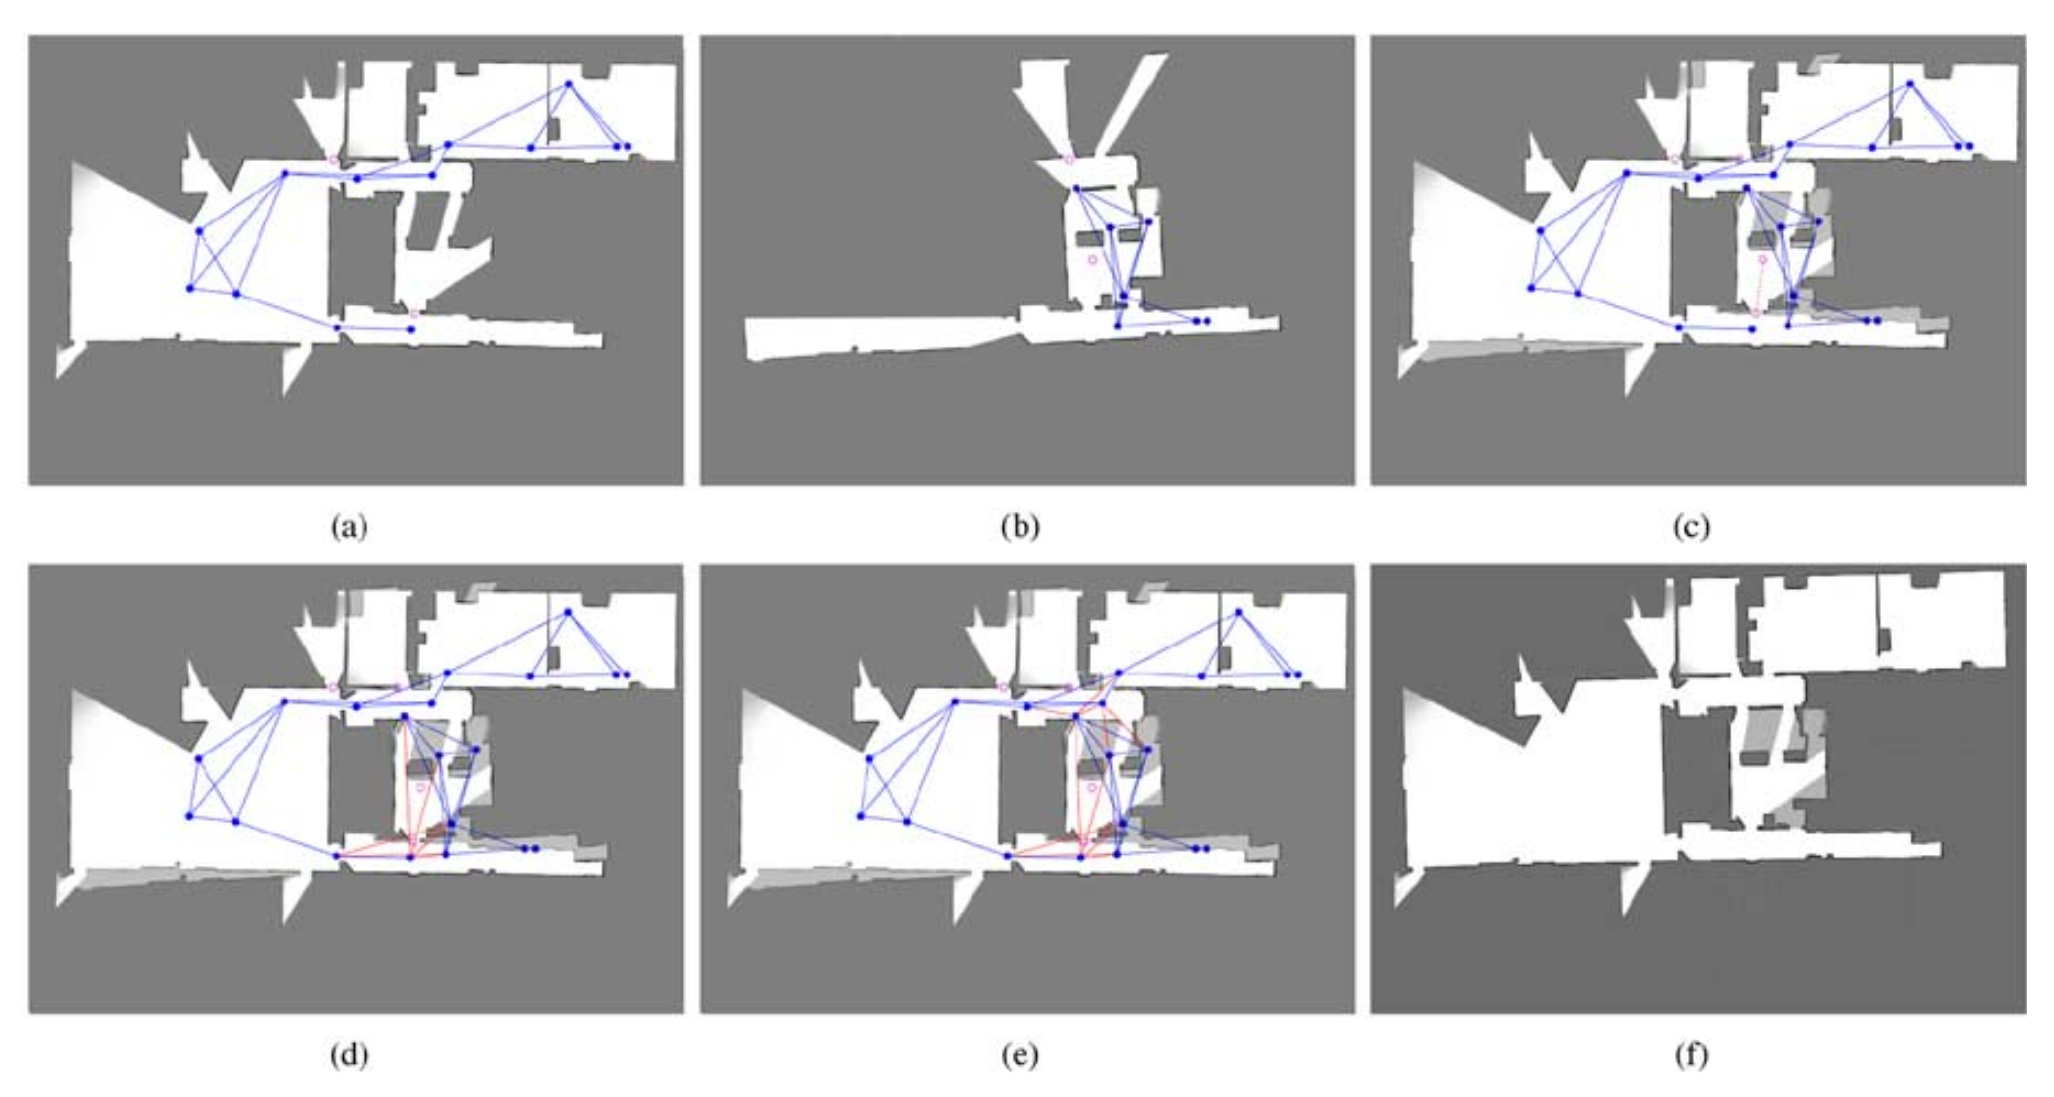
\includegraphics[scale=0.1]{images/manifold}
  \caption{Map construction process}
  \label{fig:map}
\end{figure}

%------------------------------------------------

\section{Discussion}
\subsection{Current state}
For now the algorythm is global, centralized.
The whole process is really sensitive to communication.
The map is not enhanced after first scan, I really don't like that fact.
\subsection{Possibles enhancements}
A decentralized approach can be something like that :
\begin{itemize}
  \item each robot have is own version of "global" map.
  \item adding patches is a local process made by each robot.
  \item when several robots encounter, they merge their map with loop closure
  \item after merging, they continue to notify reachables robots while adding patchs
  \item Depending on the density of the data used (point cloud, landmarks etc) it can be possible to save previous versions of the map in the same spirit than a version manager like git. It can help to find more accurate map later.
\end{itemize}

\printbibliography
\end{document}
